%%
%% Capítulo 4: Nurse: uma aplicação para produtividade em vacinações
%%

\mychapter{Nurse: uma aplicação para produtividade em vacinações}
\label{Cap:Implementacao}
Nessa seção, os requisitos e casos de usos da aplicação serão descritos. Além disso, será apresentada a arquitetura escolhida para a aplicação, tanto no sentido das camadas hierárquicas de responsabilidade \cite{Faust2020}, quanto na divisão de pastas e subpastas dos arquivos que compõem o código em módulos e, por fim, as telas do aplicativo e os pacotes utilizados para o desenvolvimento das funcionalidades serão mostrados.

O projeto foi desenvolvido utilizando a linguagem de programação \textit{Dart}, com o \textit{framework Flutter}. O seu repositório pode ser encontrado no \textit{GitHub}, em \url{https://github.com/Dojak220/nurse}. A documentação, que inclui a versão dessa monografia em formato \textit{pdf} e o seu respectivo projeto em \LaTeX também pode ser encontrada no \textit{Github}, em \url{https://github.com/Dojak220/nurse-docs}.
% [A fazer] Criar um GitHub Pages \url{https://dojak220.github.io/nurse/}.

\section{Requisitos do Sistema}
\label{cap4:Sec:Requisitos}

Os requisitos da aplicação foram definidos de acordo com a análise feita a partir do problema identificado e com os objetivos descritos nas seções \ref{cap1:Sec:Problema} e \ref{cap1:Sec:Objetivos}, respectivamente. Em suma, eles foram definidos com o intuito de suprir as necessidade de seus usuários com base naquilo que quer-se resolver. Esses requisitos, por sua vez, podem ser divididos em três tipos: funcionais, não funcionais e de domínio. Certos requisitos podem não estar claramente definidos como uma das três opções acima e, em alguns casos, um dado requisito pode se subdividir em mais requisitos menores e de tipos diferentes daquele que o originou \cite{sommerville2007engineering}. 

\subsection{Requisitos Funcionais}
\label{cap4:Subsec:RequisitosFuncionais}
Os requisitos funcionais (RF) são aqueles que descrevem as funcionalidades que o sistema deve possuir para atender às necessidades do usuário \cite{sommerville2007engineering}. A seguir (tabela \ref{tab:rf}), são apresentados os requisitos funcionais do sistema e os detalhes para alguns deles podem ser encontrados no apêndice \ref{apendice:requisitos_funcionais_detalhados}.

\begin{table}[ht!]
  \centering
  {\rowcolors{0}{white}{green!20}
  \begin{tabularx}{\textwidth}{
    | >{\centering\arraybackslash}m{0.10\textwidth} 
    | >{\centering\arraybackslash}X 
    | >{\raggedright\arraybackslash}X | }
    \hline
    \rowcolor{green!100}
    \textbf{Código} & \textbf{Requisito} & \textbf{Descrição} \\ \hline \hline
    RF01  &  Cadastrar entidades              & Permitir que o usuário cadastre novas entidades (sub-requisitos na tabela \ref{tab:rf01_detalhe}) \\ \hline
    RF02  &  Visualizar entidades cadastradas & Permitir que o usuário visualize as entidades cadastradas e seus detalhes (sub-requisitos na tabela \ref{tab:rf02_detalhe}) \\ \hline
    RF03  &  Editar entidades                 & Permitir que o usuário edite entidades já cadastradas seguindo fluxo análogo ao cadastro de nova entidade, porém, com campos pré-preenchidos \\ \hline
    RF04  &  Gerar tabela de vacinações       & Permitir que o usuário gere uma tabela de vacinações para exportação (sub-requisitos na tabela \ref{tab:rf04_detalhe}) \\ \hline
  \end{tabularx}}
\caption{Requisitos funcionais da aplicação Nurse}
\label{tab:rf}
\end{table}

\subsection{Requisitos Não Funcionais}
\label{cap4:Subsec:RequisitosNaoFuncionais}

Os requisitos não funcionais (RNF) são aqueles que descrevem as características do sistema que não são diretamente implementadas como uma funcionalidade específica na aplicação, mas que são importantes para o seu funcionamento, como o nível de confiabilidade da aplicação, performance e segurança. Além disso, são esses requisitos que apresentam as restrições inerentes à aplicação \cite{sommerville2007engineering}. A seguir (tabela \ref{tab:rnf}), são apresentados os requisitos não funcionais do sistema.

\begin{table}[ht!]
  \centering
  {\rowcolors{0}{white}{green!20}
  \begin{tabularx}{\textwidth}{
    | >{\centering\arraybackslash}m{0.10\textwidth} 
    | >{\centering\arraybackslash}X 
    | >{\raggedright\arraybackslash}X | }
    \hline
    \rowcolor{green!100}
    \textbf{Código} & \textbf{Requisito} & \textbf{Descrição} \\ \hline \hline
    RNF01  &  Correta estrutura dos dados              & Garantir que os dados fornecidos pelo usuário sejam aceitos e salvos apenas se seguirem as especificações e regras relativas a eles (por exemplo, CPF que deve seguir um conjunto de regras para ser considerado válido)   \\ \hline
    RNF02  &  Dados em planilha & Apenas os dados referentes às vacinações devem postos em uma planilha e esta deve seguir o formato apresentado na seção \ref{cap1:SubSec:cap1:ProcedimentoComumVacinacao}) \\ \hline
    RNF03  &  Cadastros não podem ser apagados  & As informações que forem salvas sobre qualquer uma das entidades pelo usuário não devem ser apagadas. Elas podem apenas ser alteradas (funcionalidade RF03) \\ \hline
  \end{tabularx}}
\caption{Requisitos não funcionais da aplicação Nurse}
\label{tab:rnf}
\end{table}
% [A fazer] Mostrar planilha de preenchimento da vacinação e os campos apresentados. Além disso, mostrar a planilha que deve ser exportada na plataforma.

\subsection{Casos de Uso}
\label{cap4:Subsec:CasosDeUso}

Uma das formas de representar um sistema, seu escopo e limites é através da identificação dos seus casos de uso e dos atores que interagem com o sistema \cite{schneider2001applying}. Estes atores podem ser desde pessoas a outras aplicações e os casos de uso descrevem o que os atores querem que o sistema realize. A seguir, na Figura \ref{fig:casos_de_uso}, é apresentado o diagrama dos casos de uso da aplicação Nurse e, logo abaixo, a tabela \ref{tab:actors} com a descrição dos atores envolvidos.

\begin{figure}[!ht]
  \centering
  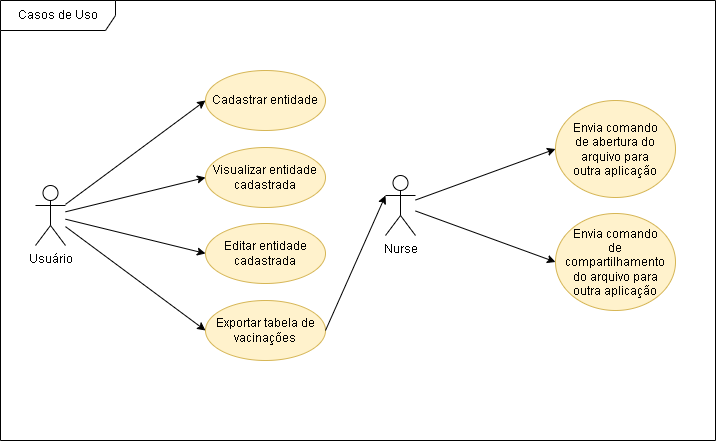
\includegraphics[width=\textwidth]{figuras/cap4/4_1_3_use_cases.png}
  \caption{Diagrama de casos de uso da aplicação Nurse}
  \label{fig:casos_de_uso}
\end{figure}

\begin{table}[ht!]
  \centering
  {\rowcolors{0}{white}{green!20}
  \begin{tabularx}{\textwidth}{
    | >{\centering\arraybackslash}m{0.15\textwidth} 
    | >{\centering\arraybackslash}X |}
    \hline
    \rowcolor{green!100}
    \textbf{Ator} & \textbf{Descrição} \\ \hline \hline
    Usuário & Usuário que utiliza a aplicação Nurse para gerenciar os dados das vacinações realizadas \\ \hline
    Nurse & É a própria aplicação utilizada, mas que também realiza chamada para abertura e/ou compartilhamento de planilhas em outras aplicações \\ \hline
  \end{tabularx}}
\caption{Descrição dos atores envolvidos na aplicação Nurse}
\label{tab:actors}
\end{table}

\section{Arquitetura do Sistema}
\label{cap4:Sec:ArquiteturaSistema}

A definição de uma arquitetura para o desenvolvimento de um projeto é essencial para que o mesmo seja desenvolvido de forma organizada e eficiente, mas também tornar a sua manutenção mais simples. Em outras palavras, o objetivo em definir uma arquitetura é diminuir os recursos humanos e, consequentemente, financeiros necessários durante todo o ciclo de vida de um projeto, desde a sua concepção até a sua manutenção, passando pelo desenvolvimento de suas funcionalidades \cite{martin2019arquitetura}. 

Para se alcançar esse objetivo, pode-se utilizar de técnicas, como as supracitadas divisão em camadas de responsabilidade e a modularização, entre outras. Além disso, é importante construir um modelo do domínio-problema da aplicação para que as complexidades inerentes a ele sejam melhor controladas \cite{evans2017domain}. O domínio, ou seja, a área na qual a aplicação Nurse está inserida e qual problema quer-se resolver, engloba do todo o conjunto de ações necessárias para realizar uma vacinação, desde o cadastro das entidades envolvidas (paciente, aplicante, vacina etc...) até a posterior exportação dos dados coletados. O modelo criado para o banco de dados é usado para modelar as entidades envolvidas e a relação entre elas, já as classes desenvolvidas para criar os arquivos a serem exportados é um exemplo da implementação no código das ações necessárias dentro desse domínio-problema.
% ref. Introdução do livro Domain-Driven Design de Eric Evans. Introdução por Martin Fowler.

\subsection{Camadas de Responsabilidade}
\label{cap4:SubSec:CamadasResponsabilidade}
A divisão em camadas hierárquicas de responsabilidade tem como objetivo dividir o projeto em partes menores, cada uma com uma responsabilidade específica e de forma a torná-las o mais independente possível entre elas \cite{Faust2020} e, dessa forma, diminuir o acoplamento e aumentar a coesão das classes. Um exemplo desse tipo de arquitetura é o sistema MVC (Model-View-Controller), que divide o projeto em três camadas: a \textbf{camada de modelo}, que contém as classes que representam as entidades do domínio-problema e gerencia os dados associados a elas; a \textbf{camada de visualização}, que contém as classes que representam as telas da aplicação e gerenciam as suas mudanças textuais e gráficas; e a \textbf{camada de controle}, que contém as classes que intermedeiam as outras duas camadas ao interpretar as ações do usuário e enviar comandos às classes do modelo e/ou da visualização para realizar quaisquer mudanças necessárias \cite{burbeck1987mvc}.

% [A fazer] Colocar as informações dessa parte na lista de itens, favorecendo uma explicação mais detalhada sobre cada uma das camadas. Talvez até subtópicos.
Essa divisão pode ser realizada em \textit{n} camadas. No caso da aplicação Nurse, dividiu-se o projeto em cinco, como mostrado na figura \ref{fig:4_1_1_camadas_nurse}.

\begin{figure}[!ht]
  \centering
  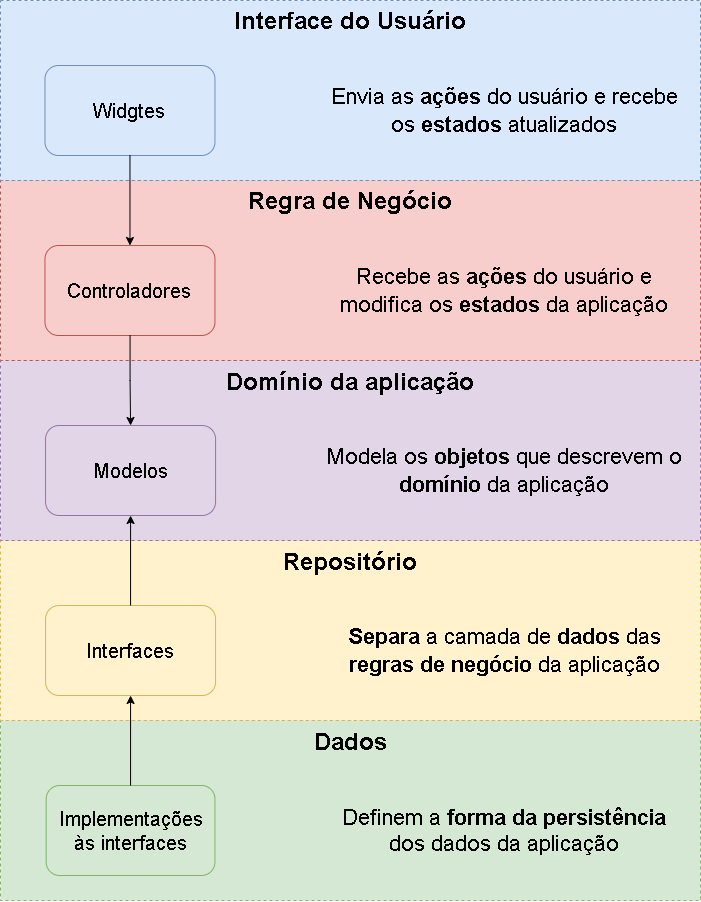
\includegraphics[width=0.6\textwidth]{figuras/cap4/4_1_1_camadas_nurse.png}
  \caption{Camadas da aplicação \textbf{Nurse} e suas dependências}
  \label{fig:4_1_1_camadas_nurse}
\end{figure}

\subsubsection{Interface do Usuário}
\label{cap4:SubSubSec:UI}
Engloba todos os elementos (\textit{widgets}) visuais e de interação com o usuários, como campos de texto ou botões, cores, imagens, ícones, etc... Essa camada é responsável por receber os comandos do usuário e enviar comandos para as outras camadas, como a camada de controle, para que as ações necessárias sejam realizadas. Além disso, é responsável por gerenciar as mudanças de estado da interface, como a mudança de cor de um botão ao ser clicado, por exemplo. As telas apresentadas na seção seguinte (\ref{cap4:Sec:Telas}) mostram esses elementos com mais detalhes.

\subsubsection{Camada de Regra de Negócio}
\label{cap4:SubSubSec:RegraNegocio}
% [A revisar]
A camada de controle recebe as ações tomadas pelo usuário na camada de interface e toma decisões a partir delas. Essas decisões são tomadas com base nas regras de negócio da aplicação (daí o nome da camada). Essas regras são implementadas em classes que fazem parte dessa camada, aqui nomeadas como \textbf{Controladores}.

Por exemplo, a classe \textit{AddPatientFormController} é responsável por gerenciar as ações relacionadas às páginas de inserção de um novo paciente ou de edição de outro já cadastrado. Durante o preenchimento dos dados nos campos de texto e de seleção em lista suspensa, essa classe salva os dados em um objeto que representa um paciente e, ao tentar salvar, verifica-se a validade dos dados inseridos pelo usuário e se esse cadastro já não havia sido realizado. Caso algum desses requisitos não seja atendido, um estado de erro é enviado à camada anterior para que esta apresente uma mensagem ao usuário, caso contrário, o objeto (um novo paciente, nesse exemplo) é enviado à camada responsável por salvá-lo no banco de dados e o usuário é redirecionado para a página de listagem de pacientes, onde poderá ver o novo item adicionado.

Vale ressaltar que essa validação, assim como o salvamento dos dados, não é responsabilidade dos controladores, então essas ações são delegadas a outras classes e/ou camadas e apenas os resultados que interessam aos controladores são retornados. A seguir, no trecho de código \ref{lst:patient_form_controller} são apresentados alguns detalhes da classe \textit{AddPatientFormController}, ressaltando o uso do \textit{MobX} e os métodos que conectam as camadas adjacentes à da regra de negócio.

% [A fazer] Colocar o código da classe PatientFormController
\begin{lstlisting}[caption={Trechos da classe \textit{PatientFormController}}, label={lst:patient_form_controller}]
  class AddPatientFormController = _AddPatientFormControllerBase
      with _$AddPatientFormController;

  abstract class _AddPatientFormControllerBase extends AddFormController
      with Store {
    // ...

    @observable
    ObservableList<Locality> localities =
      ObservableList.of(List<Locality>.empty(growable: true));

    @observable
    ObservableList<PriorityCategory> categories =
      ObservableList.of(List<PriorityCategory>.empty(growable: true));
      
    @observable
    PatientStore patientStore = PatientStore();

    final Patient? initialPatientInfo;

    _AddPatientFormControllerBase(this.initialPatientInfo) {
      if (initialPatientInfo != null) {
        patientStore.setInfo(initialPatientInfo!);
      }
  
      getLocalities();
      getPriorityCategories();
    }

    @action
    Future<List<Locality>> getLocalities() async {
      final localities = await _localityRepository.getLocalities();

      this.localities
        ..clear()
        ..addAll(await _localityRepository.getLocalities());

      return localities;
    }

    @action
    Future<List<PriorityCategory>> getPriorityCategories() async {
      // ...
    }

    @override
    Future<bool> saveInfo() async {
      if (submitForm(formKey)) {
        final PatientStore p = patientStore;
        
        // ...

      } else {
        return false;
      }
    }

    @override
    Future<bool> updateInfo() async {
      if (initialPatientInfo == null) return false;

      if (submitForm(formKey)) {
        final PatientStore p = patientStore;
        
        // ...

      } else {
        return false;
      }
    }

    // ...
  }
\end{lstlisting}

Inicialmente, na declaração da classe, utilizou-se o padrão sugerido na própria documentação do \textit{mobx} no Flutter para geração automática de código por meio do pacote de desenvolvimento \textit{mobx\_codegen} \cite{mobx_core_concepts}. Essa geração torna mais simples a utilização dos recursos do \textit{MobX}, como os \textit{\textbf{Observables}} e \textit{\textbf{Actions}} e, por isso, foi utilizada. Adiciona-se à declaração, uma extensão à classe abstrata \textit{AddFormController}, responsável por definir métodos comuns a todas as classes de controle de formulários de inserção de dados como, por exemplo, os métodos \textit{saveInfo} e \textit{updateInfo}.

Em seguida, podemos observar três propriedades observáveis, sendo duas listas e um objeto do tipo \textbf{\textit{PatientStore}} que, por sua vez, também possui propriedades observáveis internamente. É nessa última que estão os valores sobre o paciente, enviados pelo usuário na interface, como mostra o trecho de código \ref{lst:patient_store}. Nesse exemplo são mostradas algumas propriedades e métodos responsável por atualizá-las.

\begin{lstlisting}[caption={Trechos da classe \textit{PatientStore}}, label={lst:patient_store}]
  class PatientStore = _PatientStoreBase with _$PatientStore;

  abstract class _PatientStoreBase with Store {
    @observable
    Locality? selectedLocality;

    @observable
    String? cns;
  
    @observable
    String? name;

    ...outras propriedades

    @action
    void setLocality(Locality? value) => selectedLocality = value;
  
    @action
    void setCns(String value) => cns = value;
  
    @action
    void setName(String value) => name = value;
  
    // ...outros metodos
  
    @action
    void setInfo(Patient patient) {
      selectedLocality = patient.person.locality;
      selectedBirthDate = patient.person.birthDate;
      cns = patient.cns;
      name = patient.person.name;

      // ...
    }
  
    @action
    void clearAllInfo() {
      selectedLocality = null;
      selectedBirthDate = null;
      cns = null;
      name = null;

      // ...
    }
  }
  
\end{lstlisting}

De volta à listagem \ref{lst:patient_form_controller}, logo após as propriedades observáveis, temos os métodos \textbf{\textit{getLocalities}} e \textit{\textbf{getPriorityCategories}}, que agem como ações (marcadas com o \textit{@action}) e são responsáveis por buscar as informações necessárias para preencher as listas usadas para seleção de localidade e categoria de prioridade, respectivamente. Esses métodos são chamados no construtor da classe (simplificado nesse trecho de código), que recebe como parâmetro um objeto do tipo \textit{Patient}, que é utilizado para preencher os campos do formulário quando o usuário deseja editar um paciente já existente. Essa classe também possui os métodos \textit{saveInfo} e \textit{updateInfo} que são responsáveis por salvar e atualizar os dados do paciente no banco de dados, respectivamente.

\subsubsection{Domínio da Aplicação}
\label{cap4:SubSubSec:Dominio}
Nessa camada estão as classes que representam as entidades do domínio-problema da aplicação. Observa-se que essa camada não depende de nenhuma outra e pode ser considerada aquela que vai dirigir as implementações das demais \cite{evans2017domain}. Essas classes são definidas com base no mesmo modelo descrito, com mais detalhes, na seção \ref{cap4:SubSec:DiagramaClasses}. No trecho de código \ref{lst:vaccine_model} a seguir, é possível ver como a classe \textit{Vaccine}, que modela uma vacina presente no domínio do problema, é implementada.

\begin{lstlisting}[caption={Trecho da implementação da classe \textbf{Vaccine}}, label={lst:vaccine_model}]
  class Vaccine implements GenericModel {
    @override
    final int? id;
    final String sipniCode;
    final String name;
    final String laboratory;

    Vaccine({
      this.id,
      required String sipniCode,
      required String name,
      required String laboratory,
    })  : sipniCode = sipniCode.trim(),
          name = name.trim(),
          laboratory = laboratory.trim() {
      _validateVaccine();
    }

    void _validateVaccine() {
      if (id != null) Validator.validate(ValidatorType.id, id!);
      Validator.validateAll([
        ValidationPair(ValidatorType.numericalString, sipniCode),
        ValidationPair(ValidatorType.name, name),
        ValidationPair(ValidatorType.name, laboratory),
      ]);
    }
    ...
  }
\end{lstlisting}

A partir dessa classe, podemos verificar aquilo que compõe essa camada. A classe em si representa o que seria a vacina aplicada pelo profissional da saúde dentro de um processo de vacinação a um paciente e, portanto, é uma entidade do domínio-problema. Interno a essa classe estão os atributos que representam as informações que a vacina possui, como o seu nome, seu código SIPNI e o laboratório que a produziu. Além disso, é possível ver que a classe implementa a interface \textit{GenericModel}, que é uma interface que define os atributos e métodos que devem ser implementados por todas as classes que representam entidades do domínio-problema. Essa interface é definida no arquivo \textit{generic\_model.dart} e pode ser vista no trecho de código \ref{lst:generic_model} a seguir.

\begin{lstlisting}[caption={Interface \textbf{GenericModel}}, label={lst:generic_model}]
  abstract class GenericModel {
    final int? id;
  
    GenericModel(this.id);
  
    Map<String, dynamic> toMap();
  }
\end{lstlisting}

A classe \textit{Vaccine} também implementa os métodos \textit{fromMap} e \textit{toMap}, que são responsáveis por converter um objeto dessa classe em um \textit{Map} e vice-versa. Esses métodos são utilizados pelos repositórios para salvar e recuperar os dados.

Há, também, um processo de validação realizado pelo \textbf{\textit{Validator}}. Essa classe de suporte transita entre as camadas de domínio e de regra de negócio, pois ela é utilizada pelos \textit{models} para garantir que as informações que estão tentando ser cadastradas são válidas de acordo com as regras que definem o domínio-problema. Caso haja algum erro, essa informação é devolvida enviada para a camada de regra de negócio.

\subsubsection{Camada de Repositório}
\label{cap4:SubSubSec:Repositorio}

% [A revisar]
A camada de repositório separa a camada de dados da camada da regra de negócio \cite{Faust2020} \cite{andrea_repositories}. Ela é responsável por abstrair a forma como os dados são armazenados, permitindo que a aplicação seja portada para diferentes bancos de dados ou para API's sem que seja necessário alterar a regra de negócio. Essa camada é composta por classes abstratas (\ref{lst:campaign_repository}) que definem uma interface com os métodos a serem implementados pelas classes que utilizam-se dessa interface (\ref{lst:database_campaign_repository}). A seguir, no trecho de código \ref{lst:campaign_repository}, é apresentada a interface \textbf{CampaignRepository} e sua implementação para uso de banco de dados, \textbf{DatabaseCampaignRepository}, pode ser vista no trecho de código \ref{lst:database_campaign_repository}, na seção \ref{cap4:SubSubSec:Dados}.

\begin{lstlisting}[caption={Interface \textbf{CampaignRepository}}, label={lst:campaign_repository}]
  abstract class CampaignRepository {
    Future<int> createCampaign(Campaign campaign);
    Future<int> deleteCampaign(int id);
    Future<Campaign> getCampaignById(int id);
    Future<Campaign> getCampaignByTitle(String title);
    Future<List<Campaign>> getCampaigns();
    Future<int> updateCampaign(Campaign campaign);
  }
\end{lstlisting}

Pode-se observar que a classe \textbf{CampaignRepository} define seis funções relacionadas à criação, atualização, busca e remoção de campanhas de vacinação. Contudo, ela não determina como essas funções devem ser implementadas, apenas que as sejam. Dentro da camada de regra de negócio, a dependência, as classes recebem como dependência um objeto do tipo \textbf{CampaignRepository} e, dessa forma, não precisam se preocupar com a forma como os dados serão armazenados, mas apenas garantir que a chamada às funções de armazenamento sigam a assinatura da interface definida. No trecho de código a seguir (\ref{lst:campaign_repository_usage}) é apresentado um exemplo de de uso.

\begin{lstlisting}[caption={Exemplo de uso da interface \textbf{CampaignRepository}}, label={lst:campaign_repository_usage}]
  class AddCampaignFormController extends AddFormController {
    final CampaignRepository _repository;
    
    ...
  
    AddCampaignFormController(
        [CampaignRepository? campaignRepository])
        : _repository = campaignRepository ?? DatabaseCampaignRepository() {...}
    }

    ...
  }
\end{lstlisting}

A classe de controle da adição de novas campanhas de vacinação recebe o repositório \textbf{CampaignRepository} como parâmetro no construtor. Dessa forma, ao criar-se uma instância desse controlador, é possível passar um repositório diferente, como um repositório que armazena os dados em um banco de dados relacional ou outro que utiliza um banco de dados não relacional. Como, nesse projeto, utiliza-se apenas uma forma de armazenamento, definiu-se como repositório padrão o \textbf{DatabaseCampaignRepository}, contudo, ainda é possível passar outros tipos de repositório como parâmetro sem a necessidade de mudar nenhuma linha de código dentro do controlador.

\subsubsection{Camada de Dados}
\label{cap4:SubSubSec:Dados}

É nessa camada que serão realizadas as implementações dos repositórios definidos na camada de repositório. Nesse projeto, foi utilizado o banco de dados SQLite para armazenar os dados, como será melhor explicado nas seções \ref{cap4:Subsec:sqflite-sqlcipher-package} e \ref{cap4:Sec:PersistenciaDados}.

No trecho de código abaixo (\ref{lst:database_campaign_repository}) é apresentada a implementação do repositório \textbf{DatabaseCampaignRepository}. Pode-se observar que a classe implementa a interface \textbf{CampaignRepository} e, portanto, deve implementar todos os métodos definidos nessa interface (apenas dois dos métodos foram apresentados aqui, pois os outros possuem uma estrutura análoga a estes). Além disso, a classe herda de \textbf{DatabaseInterface} que, por sua vez, define métodos de acesso ao banco de dados que serão utilizados por todas as classes concretas de repositórios que realizam esse tipo de armazenamento.

Tanto a classe \textbf{DatabaseInterface} como a classe \textbf{DatabaseManager}, que é utilizada pela primeira, serão melhor descritas na seção \ref{cap4:Sec:UsoBancoDados}.
% [A fazer]

\begin{lstlisting}[caption={Implementação na classe \textbf{DatabaseCampaignRepository} da interface \textbf{CampaignRepository}}, label={lst:database_campaign_repository}]
  class DatabaseCampaignRepository extends DatabaseInterface
      implements CampaignRepository {
    // ignore: constant_identifier_names
    static const String TABLE = "Campaign";

    DatabaseCampaignRepository([DatabaseManager? dbManager])
        : super(TABLE, dbManager);

    @override
    Future<int> createCampaign(Campaign campaign) async {
      final int result = await create(campaign.toMap());

      return result;
    }

    @override
    Future<int> deleteCampaign(int id) async {
      final int count = await delete(id);

      return count;
    }

    ... // Demais implementacoes
  }
\end{lstlisting}

% [A revisar]
% Uma das vantagens em realizar essa divisão é tornar, por exemplo, as camadas de controle e de modelo imunes às mudanças realizadas na camada de visualização, tornando esta um \textit{plug-in} daquela \cite{bob2015architecture}. Dessa forma, a camada de visualização pode ser alterada sem que a camada de negócio seja afetada em absolutamente nada, o que não pode ser afirmado no caso daquele que cumpre o papel de \textit{plug-in}.
% [A fazer]
% retirar essa explicação dos sites:
% https://priyalwalpita.medium.com/software-architecture-patterns-layered-architecture-a3b89b71a057
% https://priyalwalpita.medium.com/software-architecture-patterns-which-one-to-choose-1e368b43fe70
% e da seção 4.2.1 do artigo de Faust


\section{Telas}
\label{cap4:Sec:Telas}

% [A revisar] Programa de desenvolvimento das páginas.
Nessa seção, serão apresentadas as principais telas desenvolvidas para o aplicativo \textbf{Nurse}. O design dessa páginas foram criados por Yasmim, utilizando o \textit{software} \textbf{XD Adobe}. A seguir, serão apresentadas as telas \textbf{Home}, \textbf{listagem de entidades}, \textbf{listagem de campanhas de vacinação}, \textbf{cadastro de nova campanhas de vacinação} e a tela de \textbf{exportação de dados}.

\begin{figure}[ht!]
  \centering
          \subfloat[Tela \textbf{Home}]{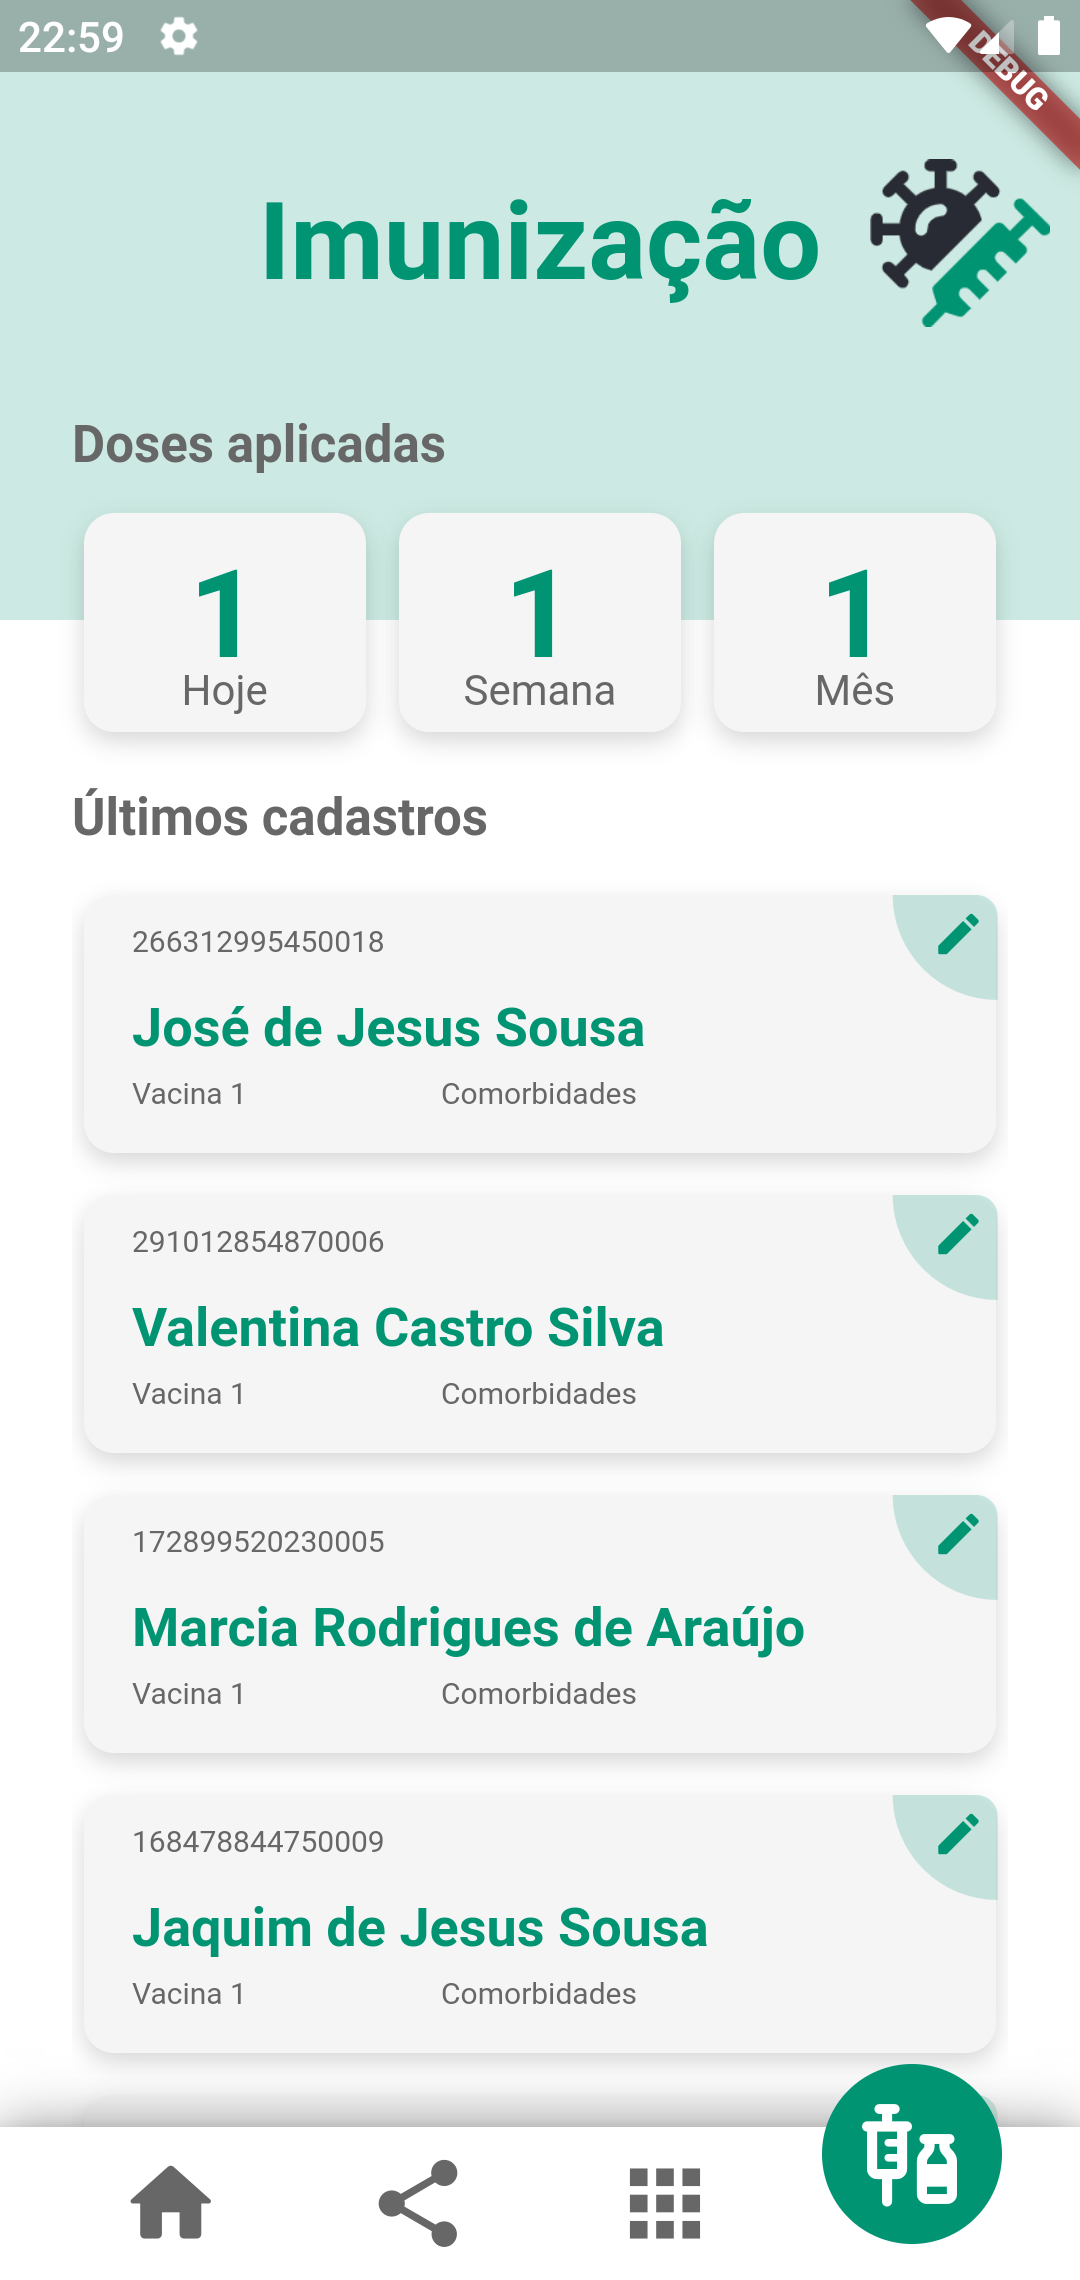
\includegraphics[width=0.29\columnwidth]{figuras/cap4/4_2_home_screen_2.png}}
            \qquad
          \subfloat[Tela \textbf{listagem de entidades}]{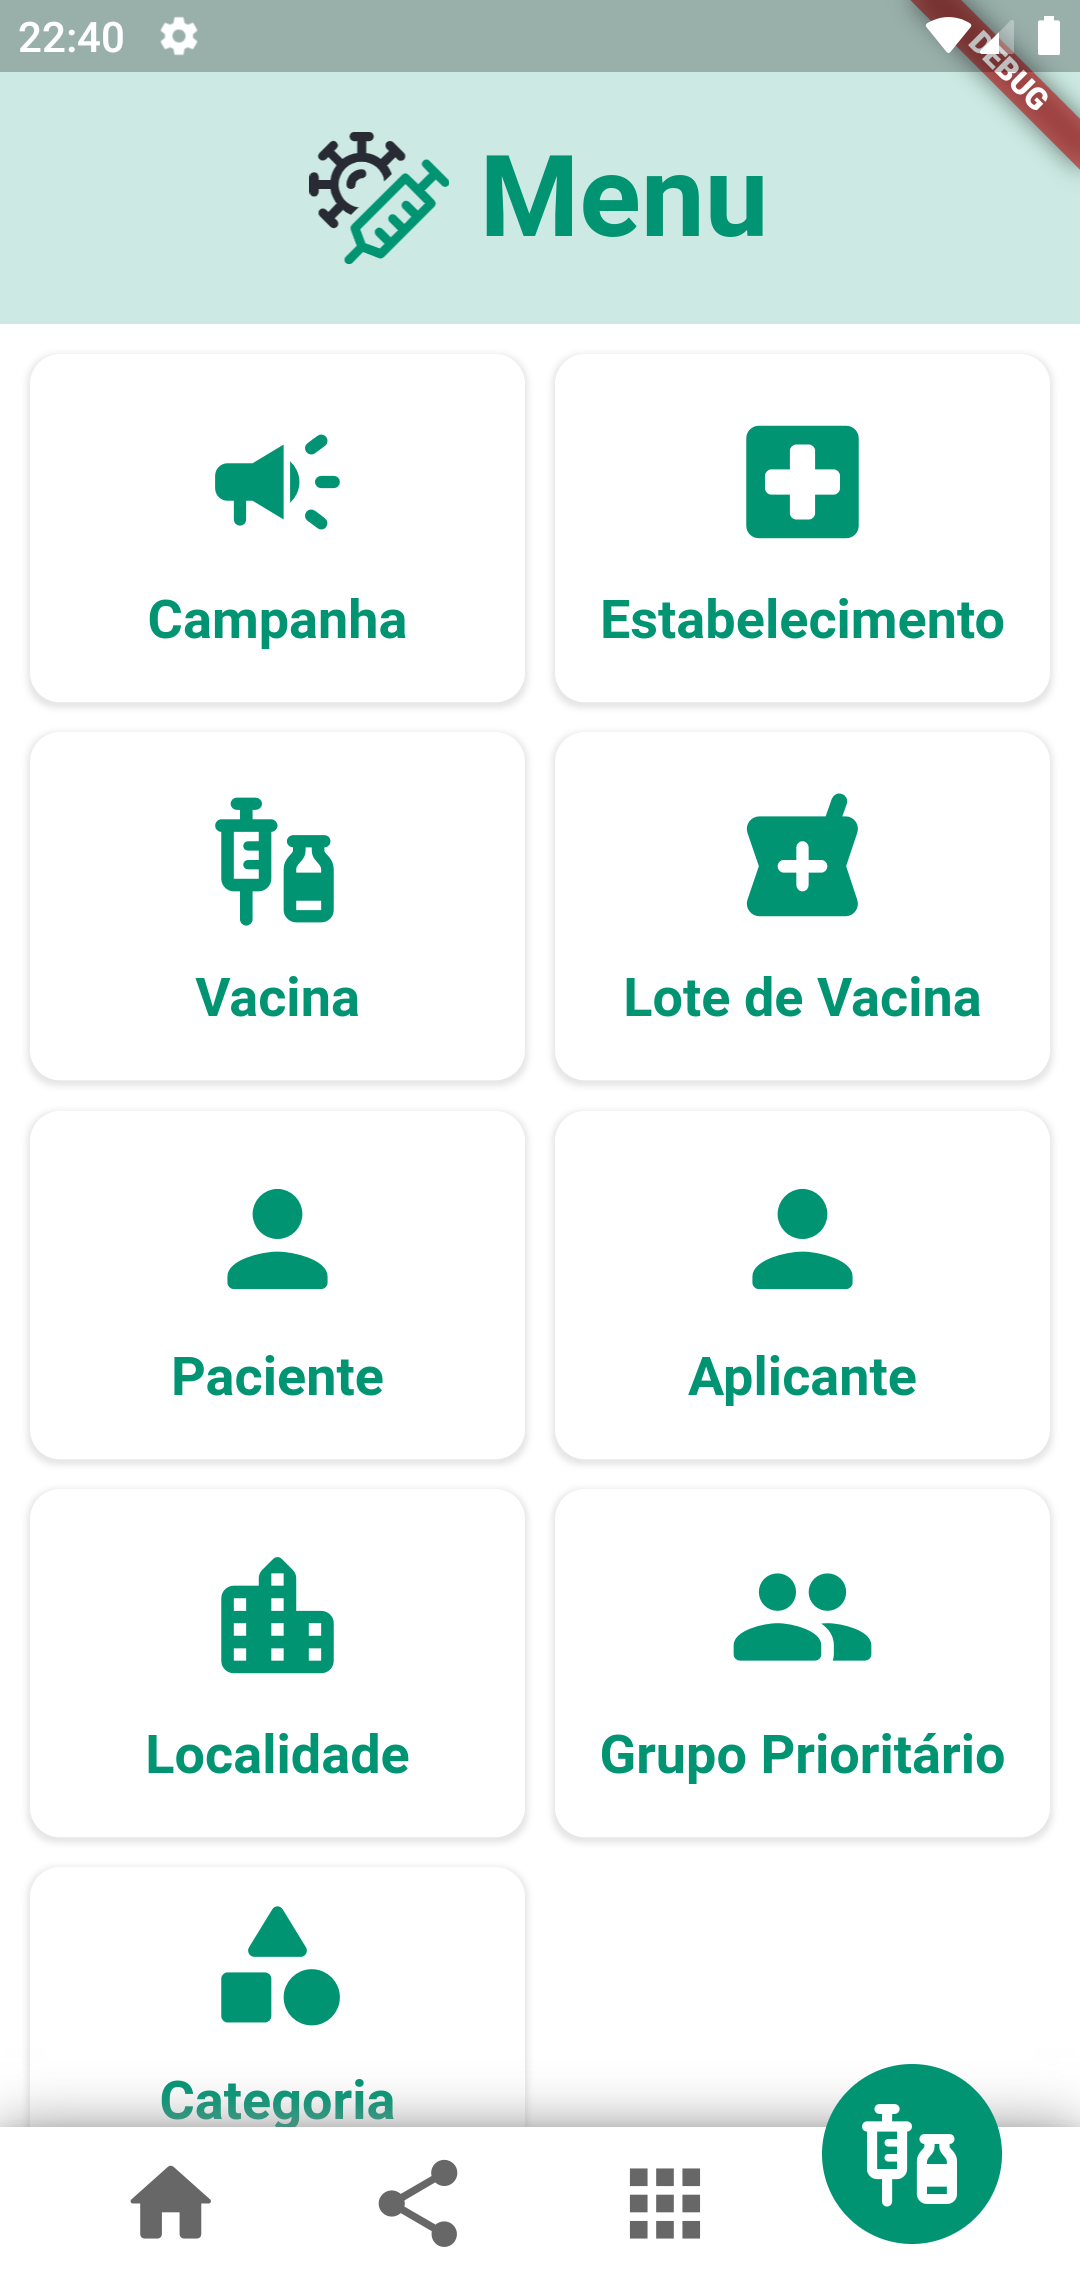
\includegraphics[width=0.29\columnwidth]{figuras/cap4/4_2_entities_screen.png}}
            \qquad
          \subfloat[Tela \textbf{exportação de dados}]{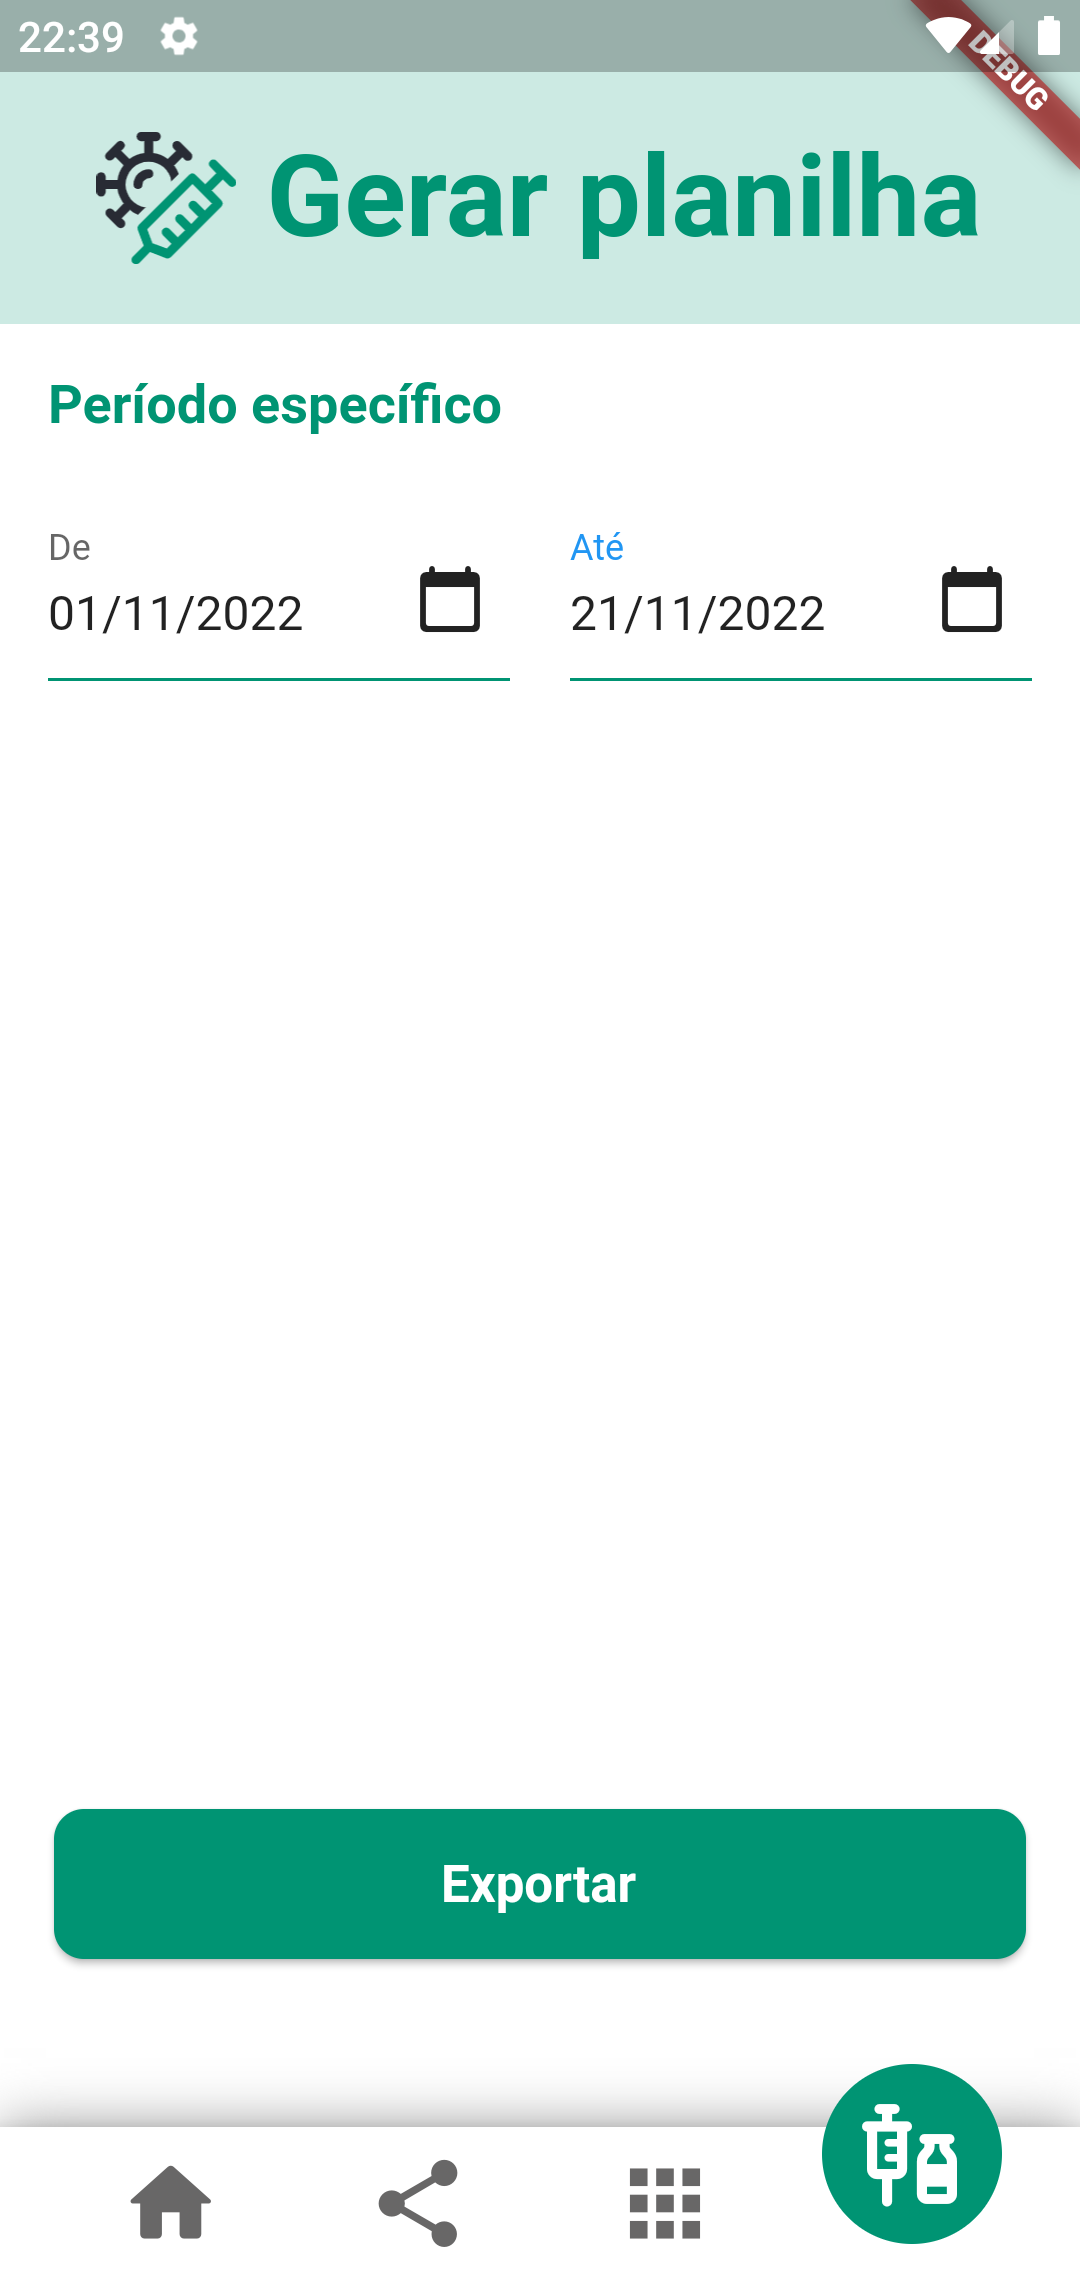
\includegraphics[width=0.29\columnwidth]{figuras/cap4/4_2_export_screen_4.png}}
    \caption[Principais telas da aplicação \textit{Nurse}]{Principais telas da aplicação \textit{Nurse}}
  % \fonte{Inserir autor aqui}
  
  \label{fig:nurse-main-screen}
\end{figure}

Todas as páginas apresentadas possuem um cabeçalho em verde que apresenta o título da página, um ícone da aplicação e, em alguns casos, um botão para voltar à página anterior. Além disso, as principais páginas possuem um rodapé que serve como sistema de navegação entre elas. Essa barra de navegação possui quatro ícones e cada um leva a uma página diferente. O primeiro ícone leva à página \textbf{Home}, o segundo à página de \textbf{listagem de entidades}, o terceiro à página de \textbf{exportação de dados} e o último e principal, ao conjunto de páginas de \textbf{cadastro de vacinação}. Essa última será apresentada em detalhes na seção \ref{cap5:SubSec:FluxoCadastroVacinacao}.

A página \textbf{Home} é a primeira página que o usuário visualiza quando abre o aplicativo. Nela, é possível ver o número de vacinas aplicadas no dia, na semana e no mês. Também é mostrado ao usuário a lista das últimas vacinas aplicadas e o paciente que as recebeu, além de outras informações sobre este.

A página \textbf{listagem de entidades} é a página que mostra ao usuário a lista de entidades cadastradas no aplicativo. Nela, é possível ver o nome da entidade e o 
ícone que a representa. Ao clicar em uma entidade, o usuário é levado à página de listagem daquela entidade.

Por fim, a página \textbf{exportação de dados} é a página que permite ao usuário exportar os dados do aplicativo referentes à vacinação para um arquivo \textbf{.csv}. Nela, o usuário pode filtrar o período que quer exportar os dados.


\begin{figure}[ht!]
  \centering
          \subfloat[Tela da lista de campanhas cadastradas]{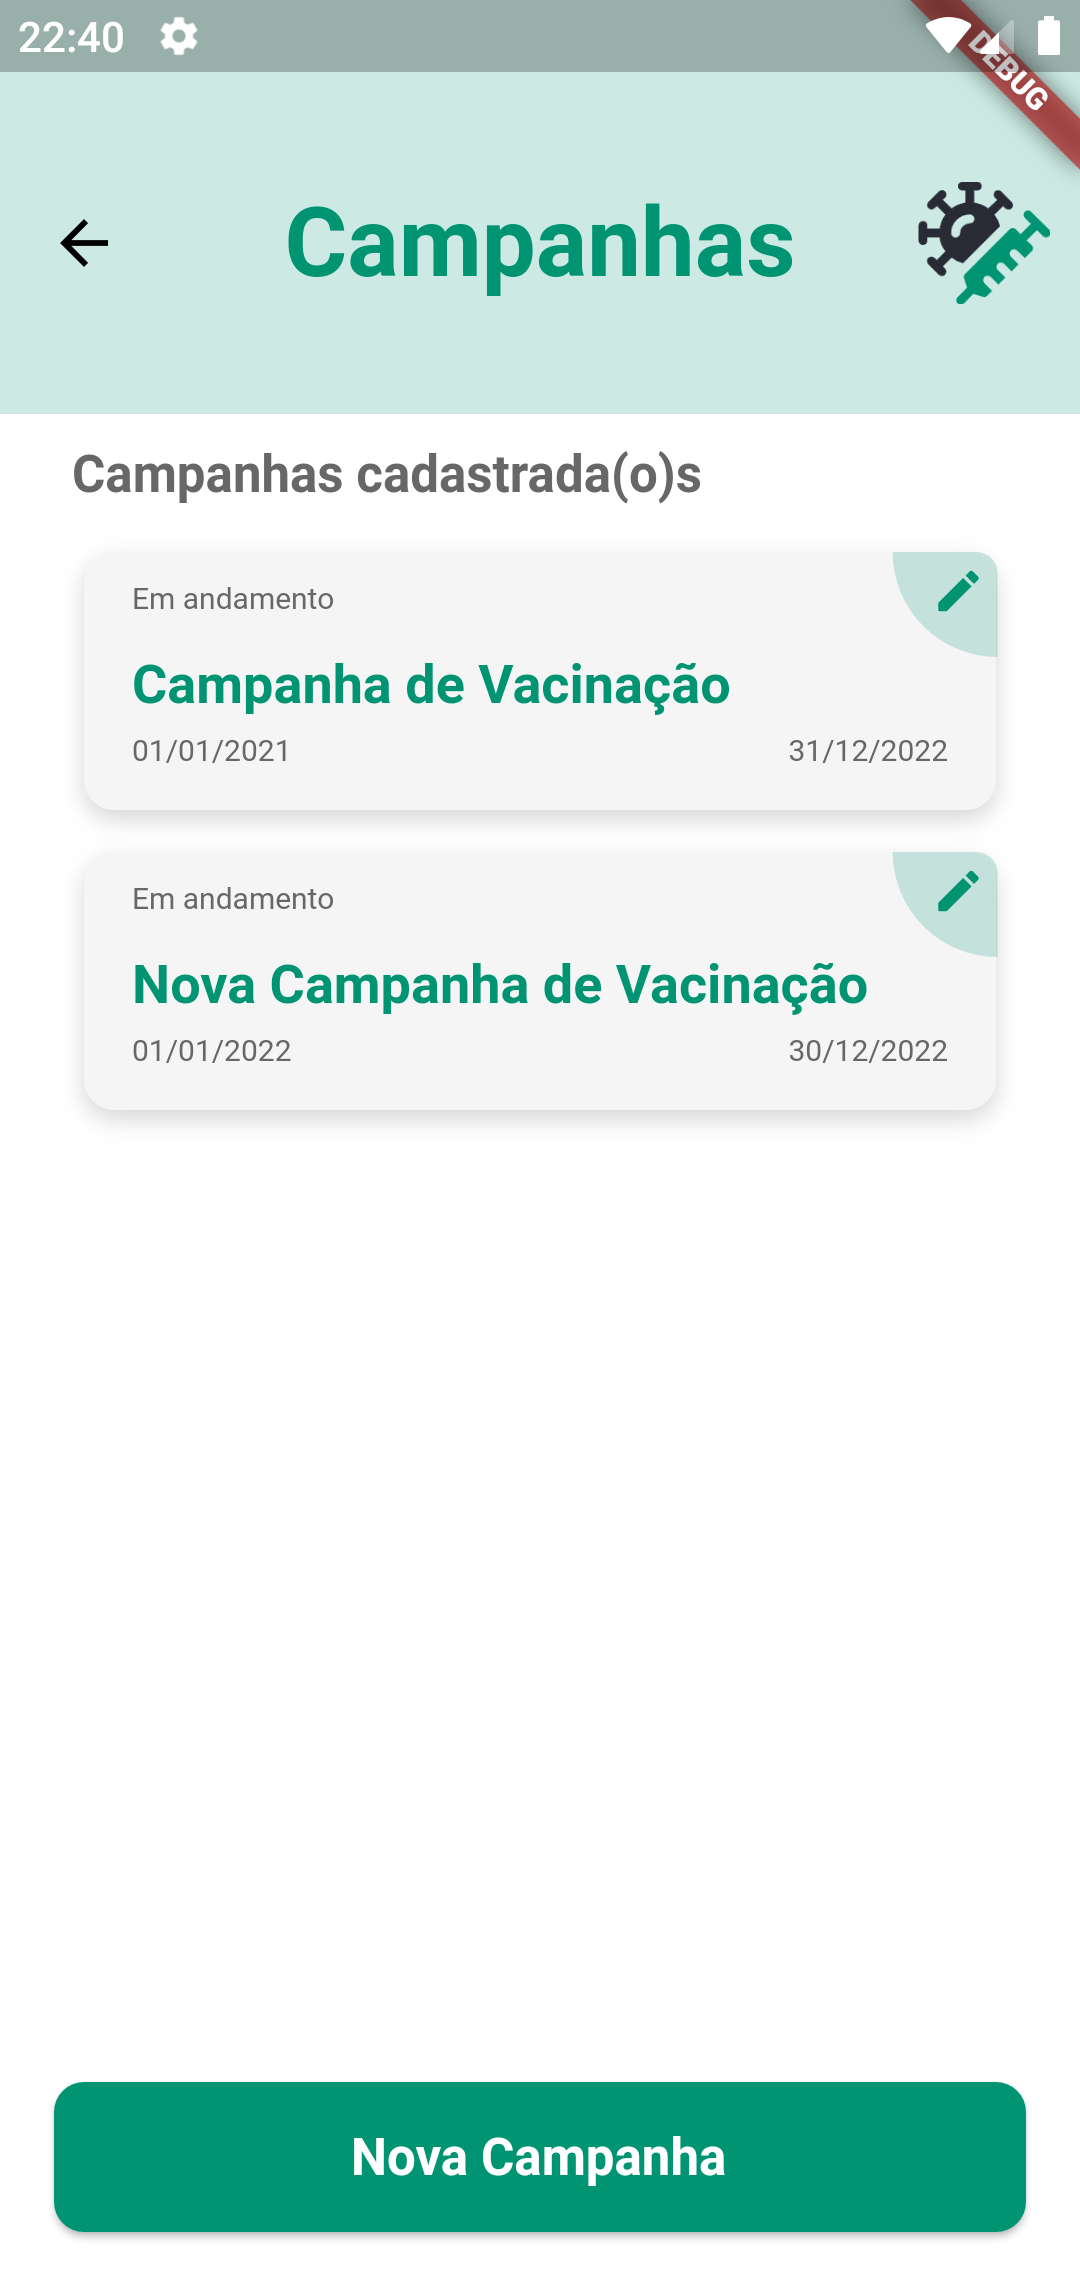
\includegraphics[width=0.29\columnwidth]{figuras/cap4/4_2_campaign_list_screen.png}}
            \qquad
          \subfloat[Tela de cadastro de nova campanha]{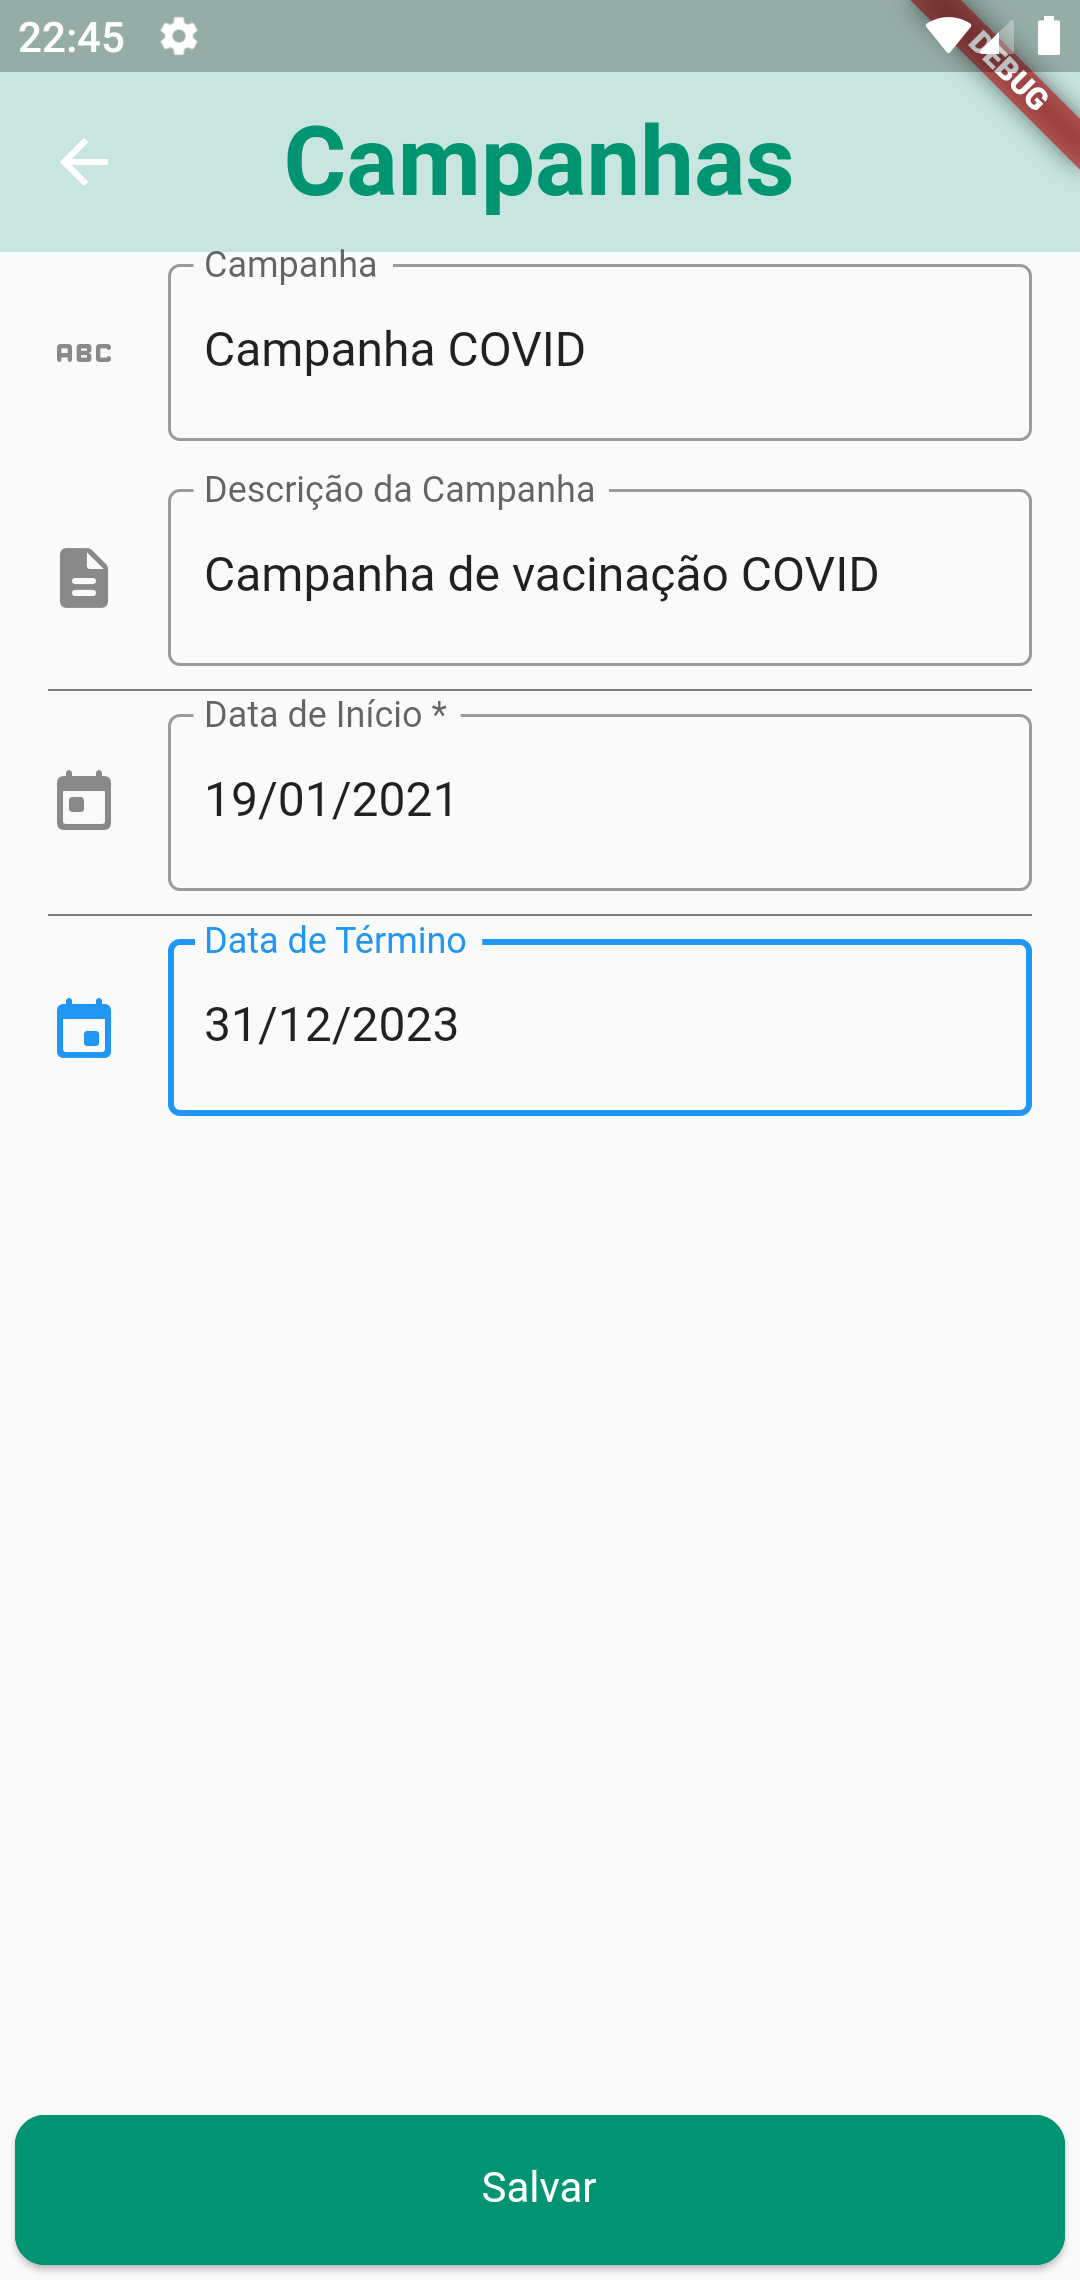
\includegraphics[width=0.29\columnwidth]{figuras/cap4/4_2_campaign_form_2.png}}
    \caption[Telas de listagem e cadastro de entidade]{Telas de listagem e cadastro de entidade}
  % \fonte{Inserir autor aqui}
  
  \label{fig:entity_list_new_entity}
\end{figure}

As telas da figura \ref{fig:entity_list_new_entity} apresentam um exemplo das telas que listam as campanhas cadastradas e o formulário de uma nova campanha. Na tela de listagem, pode-se ver duas campanhas cadastradas, um botão para novos cadastros na parte inferior na tela e um botão de edição em formato de lápis no canto superior direito de cada cartão. Esse cartão, por sua vez, apresenta as principais informações sobre aquela entidade. Por fim, quando quer-se editar um item, a página do formulário é iniciada com as informações previamente cadastradas daquele item.

\section{Pacotes e Bibliotecas}
\label{cap4:Sec:PacotesBibliotecas}

Nessa seção, serão apresentados os pacotes e bibliotecas utilizados no desenvolvimento do sistema. A tabela \ref{tab:packages}, presente no apêndice \ref{apendice:pacotes}, apresenta os pacotes utilizados no desenvolvimento do sistema e suas respectivas versões.

% [A revisar] nomes dos pacotes e bibliotecas 
Entre os pacotes e plugins utilizados, se destacam aqueles que estão relacionados com a persistência de dados (sqflite\_sqlcipher), com o gerenciamento de estado (mobx e flutter\_mobx), com a injeção de dependências (provider) e com a criação da planilha que será compartilhada (syncfusion\_flutter\_xlsio).

\subsection{\textit{Plugin}s \textit{sqflite\_sqlcipher} e \textit{sqflite}}
\label{cap4:Subsec:sqflite-sqlcipher-package}
O plugin \textit{sqflite} permite o uso do \textbf{SQLite} em aplicações \textit{Flutter} \cite{sqflite-package}. O \textit{sqflite\_sqlcipher}, por sua vez, adiciona ao primeiro a funcionalidade de criptografia do banco de dados através da biblioteca \textit{SQLCipher} \cite{sqlcipher-package}.

\subsection{Bibliotecas \textit{mobx} e \textit{flutter\_mobx}}
\label{cap4:Subsec:mobx-package}
O pacote \textit{mobx} é utilizado para a implementação do \textit{MobX} \ref{cap2:Subsec:MobX} nas aplicações em \textit{Dart/Flutter}. É com ele que o gerenciamento de estado segue o conceito de reatividade visto anteriormente, utilizando-se das suas principais classes: \textit{\textbf{Observable}}, responsável por criar o estado reativo da aplicação; e \textit{\textbf{Action}}, que definirá a função que muda esse estado. Além disso, para completar a tríade do MobX, este utiliza-se de um conjunto de reações, em forma de função, que são chamadas no momento em que o estado observado muda \cite{mobx-package}.

Em adição, têm-se o pacote \textit{flutter\_mobx}, o qual é responsável por implementar um \textit{widget} chamado \textit{\textbf{Observer}}. Este, por sua vez, garante que o seu \textit{widget} filho seja atualizado sempre que o estado relacionado a ele mude. O \textit{Observer} também é um representante das reações do MobX que, nesse caso, reage atualizando a interface do usuário \cite{flutter-mobx-package}.

No desenvolvimento da classe \textbf{HomeController}, a qual gerencia o estado observado pelos componentes da página \textbf{Home}, utilizou-se as classes \textbf{Action}, para definir a função responsável por alterar o estado observável, e \textbf{ObservableList}, uma variante da classe \textbf{Observable} para listas.

\begin{lstlisting}[caption={Uso do \textit{MobX} na classe \textbf{HomeController}}, label={lst:home_controller_mobx}]
  class HomeController {
    final ApplicationRepository applicationRepository;

    final applications = ObservableList<Application>.of(
      List<Application>.empty(growable: true),
    );

    late final fetchApplications = Action(getApplications);

    HomeController() : applicationRepository = DatabaseApplicationRepository() {
      fetchApplications();
    }

    Future<List<Application>> getApplications() async {
      final result = await applicationRepository.getApplications();
      applications.clear();
      applications.addAll(result.reversed);

      return applications;
    }

    /*...*/
  }
\end{lstlisting}

A propriedade \textit{applications} recebe, inicialmente, um \textbf{ObservableList} vazio do tipo \textit{Application} e a função \textit{fetchApplications} foi definida como a ação que modifica o estado observável, isto é, a lista de aplicações. A ação é chamada no construtor da classe \textbf{HomeController} para que a lista de aplicações seja preenchida assim que a classe for instanciada. Essa lista, por sua vez, é preenchida quando a busca realizada pela classe \textbf{ApplicationRepository} no banco de dados finaliza com sucesso.  A função \textit{fetchApplications} é chamada, também, toda vez que o usuário finaliza um novo cadastro de aplicação de vacina e é redirecionado novamente à tela inicial \textbf{Home}.

\begin{lstlisting}[caption={Uso do \textit{MobX} no \textit{widget} \textbf{Home}}, label={lst:home_page_mobx}]
  class Home extends StatelessWidget {
    /*...*/

    @override
    Widget build(BuildContext context) {
      return Scaffold(
        
        /*...*/
      
        floatingActionButton: VaccinationButton(
          newPage: "/vaccinations/new",
          onCallback: () => context.read<HomeController>().
          fetchApplications(),
        ),
        
        /*...*/

      );
    }
  }
\end{lstlisting}

No código que define a classe \textbf{Home}, mostrada parcialmente no trecho de código \ref{lst:home_page_mobx}, têm-se o \textit{widget} \textbf{Scaffold}, o qual possui a propriedade \textbf{\textit{floatingActionButton}}, que recebe o \textit{widget} \textbf{VaccinationButton}. A sua propriedade \textit{onCallback} recebe uma função que chama \textit{fetchApplications} da classe \textbf{HomeController}, para que a lista de aplicações seja atualizada. A forma como o estado é injetado na classe \textbf{Home} é explicado adiante, na \ref{cap4:Subsec:Provider}.

\subsection{Pacote \textit{provider}}
\label{cap4:Subsec:Provider}
Como descrito anteriormente, na \ref{cap2:Subsec:Provider}, o estado pode ser injetado em qualquer \textit{widget} por meio do \textit{Provider}. Sendo assim, utilizou-se o \textit{Provider} nesse projeto não para gerenciamento do estado diretamente, mas para injetar o estado gerenciado pelo \textit{mobx} em qualquer \textit{widget} da aplicação. Para isso, foi utilizado o pacote \textit{provider} \cite{provider-package}.

Desse pacote, utilizou-se duas estratégias principais:
\begin{itemize}
  \item \textbf{Provider.of<T>(context)}: injeta a classe T a partir do contexto passado via parâmetro. O Provider, então, busca na árvore de \textit{widgets} acima do \textit{widget} atual a instância mais próxima da classe T \cite{provider-package}. A seguir, no trecho de código \ref{lst:appliers_page_provider}, tem-se um exemplo de uso dessa estratégia.
  \item \textbf{context.read<T>().fn()}: assim como o anterior, utiliza-se do contexto para buscar a classe T desejada e, em seguida, faz uma chamada da função denominada \textit{fn} no exemplo, mas não passa a observar as mudanças de estado que ocorrem nessa classe, diferentemente da função \textit{watch} \cite{provider-package}. Um exemplo do seu uso foi apresentado no trecho de código \ref{lst:home_page_mobx}, no qual \textit{fetchApplications} representa a função \textit{fn} aqui descrita.
\end{itemize}

\begin{lstlisting}[caption={Uso do \textit{Provider} no \textit{widget} \textbf{Appliers}}, label={lst:appliers_page_provider}]
  class Appliers extends StatelessWidget {
    const Appliers({Key? key}) : super(key: key);

    @override
    Widget build(BuildContext context) {
      final controller = Provider.of<AppliersPageController>(context);
      /*...*/

      return EntityList<Applier>(
        title: "Aplicantes",
        controller: controller,
        /*...*/
      );
    }
  }
\end{lstlisting}

\subsection{Biblioteca Excel (XlsIO)}
\label{cap4:Subsec:syncfusion_flutter_xlsio}
Utilizando-se do pacote \textit{syncfusion\_flutter\_xlsio}, foi possível gerar um arquivo \textit{.xlsx} a partir de uma lista de aplicações de vacina. Para isso, criou-se uma classe chamada \textbf{ExcelService} que possui dois métodos públicos: \textbf{\textit{shareExcelFile}} e \textbf{\textit{openExcelFile}}. Cada um desses métodos é chamado quando o usuário segue o fluxo apresentado na figura \ref{fig:fluxo_exportar_dados} e descrito em detalhes na seção \ref{cap5:SubSec:FluxoExportacao}.

O método \textbf{\textit{shareExcelFile}} cria um arquivo \textit{.xlsx} e permite que o usuário o compartilhe, enquanto o método \textbf{\textit{openExcelFile}} cria um arquivo \textit{.xlsx} e o abre no aplicativo de planilhas do usuário. A seguir, na figura \ref{fig:excel_service_diagram}, tem-se o fluxo de execução de ambos os métodos dentro da classe \textbf{ExcelService}.

\begin{figure}[!ht]
  \centering
  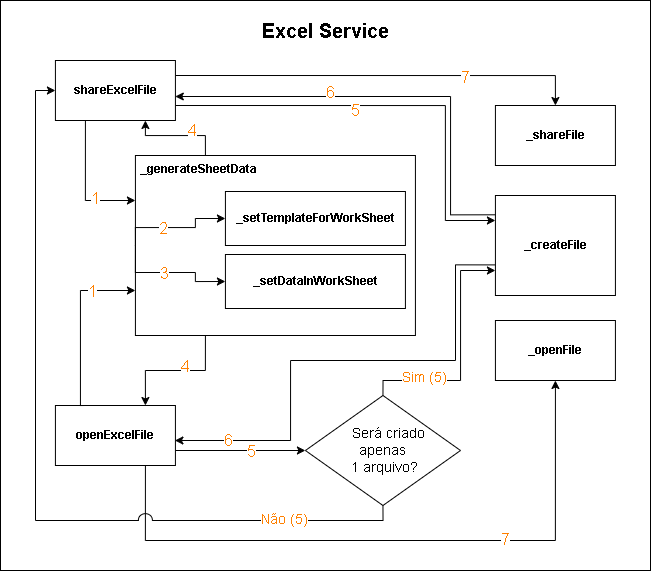
\includegraphics[width=\textwidth]{figuras/cap4/4_3_4_excel_service_diagram.png}
  \caption{Descritivo de fluxo dos métodos da classe \textbf{ExcelService}}
  \label{fig:excel_service_diagram}
\end{figure}

A ordem de execução dos métodos segue a ordem das setas numeradas. Cada um dos métodos é descrito a seguir:

\begin{itemize}
  \item \textbf{Etapa 1}: os métodos \textbf{\textit{shareExcelFile}} e \textbf{\textit{openExcelFile}} recebem como parâmetros a lista das aplicações cadastradas e o período de tempo que o usuário deseja exportar ou visualizar. Estas informações são, então, organizadas em um mapa de datas e aplicações e enviadas ao método \textbf{\textit{\_generateSheetData}}
  \item Etapas \textbf{2} e \textbf{3}: o método \textbf{\textit{\_generateSheetData}} recebe como parâmetro o mapa de datas e aplicações. A partir dos métodos \textbf{\textit{\_setTemplateForWorkSheet}} e \textbf{\textit{\_setDataInWorkSheet}}, um objeto do tipo \textbf{\textit{Workbook}} é, respectivamente estruturado e preenchido com os dados recebidos. Esse \textbf{\textit{Workbook}} é, então transformado em uma lista de bytes por meio de seu método interno \textbf{\textit{Workbook.saveAsStream()}}. Por fim, cada agrupamento de bytes é retornado em um novo mapa, onde a chave é a data das aplicações e o valor é um outro mapa de doses aplicadas e agrupamento de bytes.
  % [A fazer] Explicar na introdução porque essas planilhas devem ser separadas por data e dose
  \item \textbf{Etapa 4}: o método \textbf{\textit{\_generateSheetData}} retorna o agrupamento de bytes para as funções \textbf{\textit{shareExcelFile}} ou \textbf{\textit{openExcelFile}}, a depender de qual fluxo está sendo executado, e cada um desses agrupamentos será processado individualmente, como se segue.
  \item \textbf{Etapa 5}: para o método \textbf{\textit{openExcelFile}}, será verificado a quantidades de agrupamentos retornados. Caso seja apenas um, o arquivo será criado a partir desse agrupamento e passará ao próximo passo. Caso contrário, o fluxo desse método será finalizado e os dados serão redirecionados ao método \textbf{\textit{shareExcelFile}}. Já para este último, o fluxo é direto e cada cada conjunto de bytes separados por datas de aplicação e doses aplicadas será salvo em um arquivo.
  \item \textbf{Etapa 6}: considerando que o fluxo dos métodos \textbf{\textit{shareExcelFile}} e \textbf{\textit{openExcelFile}} foi o mesmo, ou seja, a criação dos arquivos na função \textbf{\textit{\_createFile}}, o(s) arquivo(s) recebido(s) será(ão) enviados de volta para as funções principais.
  \item \textbf{Etapa 7}: Por fim, o método \textbf{\textit{shareExcelFile}} chama a função \textbf{\textit{\_shareFile}} para compartilhar o arquivo gerado, enquanto o método \textbf{\textit{openExcelFile}} chama a função \textbf{\textit{\_openFile}} para abrir o arquivo gerado. Ambas as funções são descritas a seguir.
\end{itemize}

A função \textbf{\textit{\_shareFile}} recebe como parâmetro o arquivo gerado e, a partir da biblioteca \textit{share\_plus} e do seu método \textbf{\textit{Share.shareFiles}}, permite que o usuário compartilhe o arquivo gerado \cite{share_plus-package}. A função \textbf{\textit{\_openFile}}, por sua vez, também recebe o arquivo gerado de forma análoga à primeira função e, a partir da biblioteca \textit{open\_file} e do seu método \textbf{\textit{OpenFile.open}}, realiza a chamada a uma aplicação que possa abrir um arquivo no formato \textit{.xlsx}.

\section{Persistência de Dados}
\label{cap4:Sec:PersistenciaDados}
A persistência de dados, como descrita na seção \ref{cap2:Sec:PersistenciaDados}, é realizada por meio de um banco de dados relacional, o \textit{SQLite}. A biblioteca \textit{sqflite} é utilizada para a comunicação com o banco de dados \cite{sqflite-package}. A estrutura do banco de dados da aplicação como ela foi implementada é descrita nesta seção.

\subsection{Diagrama de Classes}
\label{cap4:SubSec:DiagramaClasses}
% ref. Cap 4 do livro Projeto de Banco de Dados Heuser
Foram definidas 9 entidades (ou classes) para a aplicação \textbf{Nurse}, as quais foram agrupadas em 3 macro-grupos: \textbf{Paciente}, \textbf{Vacinação} e \textbf{Infraestrutura}. Cada uma dessas entidades possui um identificador único, chamada chave primária (do inglês, \textit{Primary Key} (PK)) e algumas delas possuem uma ou mais chaves estrangeiras (do inglês, \textit{Foreign Key} (FK)) \cite{heuser09banco}. Além disso, cada entidade possui um ou mais atributos, que são apresentados na figura \ref{fig:diagrama_classes} e descritos a seguir.

\begin{figure}[!ht]
  \centering
  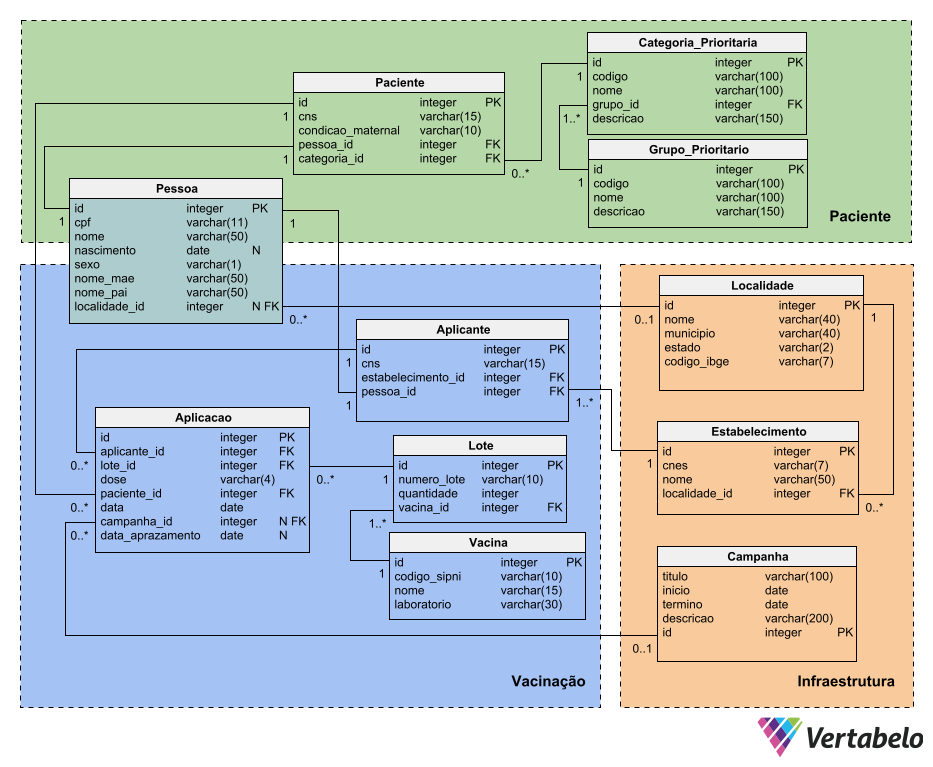
\includegraphics[width=\textwidth]{figuras/cap4/4_4_1_diagrama_classes.png}
  \caption{Diagrama de classe para a aplicação \textbf{Nurse}}
  \label{fig:diagrama_classes}
\end{figure}

\begin{itemize}
  \item \textbf{Pessoa}: é a entidade que representa uma pessoa, seja ela um paciente ou um profissional de saúde. Essa entidade possui os atributos \textbf{nome}, \textbf{cpf}, \textbf{data de nascimento}, \textbf{sexo}, \textbf{nome da mãe}, \textbf{nome do pai} e \textbf{localidade} onde reside. Essa entidade faz parte de dois grupo distintos: grupo 'Paciente' e grupo 'Aplicação', pois ela pode estar associada a um paciente ou a um aplicante da vacina.
  \item Grupo \textbf{Paciente}
  \begin{itemize}
    \item \textbf{Paciente}: é a entidade que representa um paciente. Essa entidade possui os atributos \textbf{cns} (número do Cartão Nacional de Saúde) e \textbf{condição maternal}. Além disso, a entidade \textbf{Paciente} possui duas chaves estrangeiras para as entidades \textbf{Pessoa} e \textbf{Categoria Prioritária}.
    \item \textbf{Categoria Prioritária}: é a entidade que representa uma categoria prioritária do paciente. Essa entidade possui os atributos \textbf{nome}, \textbf{código} e \textbf{descrição}. Além disso, a entidade \textbf{Categoria Prioritária} possui uma chave estrangeira para o seu \textbf{Grupo Prioritário}.
    \item \textbf{Grupo Prioritário}: é a entidade que representa um conjunto de categorias prioritárias. Um exemplo de grupo é 'Faixa Etária' e as categorias desse grupo são subconjuntos de idades (pessoas com mais de 60 anos, pessoas com menos de 18 anos etc...). Essa entidade possui os atributos \textbf{nome}, \textbf{código} e \textbf{descrição}.
  \end{itemize}
  \item Grupo \textbf{Infraestrutura}
  \begin{itemize}
    \item \textbf{Localidade}: é a entidade que representa uma localidade, seja ela uma comunidade ou uma cidade. Essa entidade possui os atributos \textbf{nome da localidade}, \textbf{município}, \textbf{estado} e \textbf{código do IBGE}.
    \item \textbf{Estabelecimento}: é a entidade que representa um estabelecimento de saúde. Essa entidade possui os atributos \textbf{nome} e \textbf{CNES} (Cadastro Nacional de Estabelecimentos de Saúde). Além disso, a entidade \textbf{Estabelecimento} possui uma chave estrangeira para a entidade \textbf{Localidade}.
    \item \textbf{Campanha}: é a entidade que representa uma campanha de vacinação. Essa entidade possui os atributos \textbf{título}, datas de \textbf{início} e \textbf{término} da campanha e sua \textbf{descrição}.
    % ref da sigla CNES: https://cnes.datasus.gov.br/ 21/11/2022 
  \end{itemize}
  \item Grupo \textbf{Vacinação}
  \begin{itemize}
    \item \textbf{Aplicante}: é a entidade que representa o profissional de saúde que realizou a aplicação da vacina no paciente. Essa entidade possui o atributo \textbf{cns}, assim como o paciente. Além disso, a entidade \textbf{Aplicante} possui duas chaves estrangeiras para as entidades \textbf{Pessoa} e \textbf{Estabelecimento}.
    \item \textbf{Vacina}: é a entidade que representa o agente imunizante que será aplicado no paciente. Essa entidade possui os atributos \textbf{nome} da vacina, seu \textbf{código SI-PNI} e o \textbf{laboratório} do fabricante.
    \item \textbf{Lote}: é a entidade que representa um lote de vacinas. Essa entidade possui os atributos \textbf{número do lote} e \textbf{quantidade de vacinas} no lote. Além disso, a entidade \textbf{Lote} possui uma chave estrangeira para a entidade \textbf{Vacina}.
    \item \textbf{Vacinação}: é a entidade central da aplicação. Ela representa todo o conjunto de informações que estão associadas ao ato de vacinar. Seus atributos representam essa centralidade. São eles: \textbf{Aplicante}, \textbf{Lote da vacina}, \textbf{Paciente} e \textbf{Campanha de vacinação}, as quais são todas chaves estrangeiras para outras tabelas. Além disso, a entidade \textbf{Vacinação} possui os atributos \textbf{dose da vacina}, \textbf{data de aplicação} e \textbf{data prazo} para próxima aplicação.
  \end{itemize}
\end{itemize}

Alguns desses atributos são obrigatórios, como o \textbf{cpf} e o \textbf{nome}, já outros podem ser deixados nulos, como é o caso do campo \textbf{sexo}, todos da tabela \textbf{Pessoa}. Além dessa, a tabela \textbf{Aplicação} também possui dois atributos chamados anuláveis, que são o identificador da tabela \textbf{Campanha} e o atributo \textbf{data de aprazamento}.

\subsection{Uso do Banco de Dados}
\label{cap4:Sec:UsoBancoDados}
















% \begin{algorithm}
% %% \SetLine
% \Entrada{$x$: vetores de valores; $y$ = $L(x)$; $p$: valor de entrada a ser calculado }
% \Saida{$s$ = $L(p)$}
% $n \leftarrow \mathtt{comprimento}(x)$\;
% $s \leftarrow 0$\;
% \Para {$i=1$ \Ate $n$} {
% 	$L \leftarrow 1$\;
% 	\Para {$j=1:1:n$} {
% 		\Se{$i \neq j$} {
% 			$L \leftarrow L* \left( \dfrac{p-x[j]}{x[i]-x[j]} \right) $
% 		}
% 	}
% 	$s \leftarrow s + L*y[i]$\;
% }
% \Retorna $s$\;
% \caption{Algoritmo para interpolação de Lagrange.}
% \label{algo:1}
% \end{algorithm}

% \begin{algorithm}
% %% \SetLine
% \Entrada{$a$: valor inicial; $b$: valor final; $n$: número de subintervalos (deve ser múltiplo de 2)  }
% \tcc{A função a ser integrada é definida em uma função denominada \texttt{f}, fora do escopo deste algoritmo.}
% \Saida{$I$ = integral de \texttt{f} entre $a$ e $b$}
% $h \leftarrow$ $\dfrac{b-a}{n}$\;
% $x[1] \leftarrow a$\;
% $y[1] \leftarrow f(a)$\;
% $I \leftarrow 0$\;
% $k \leftarrow 2$\;
% \Enqto {$k <= n$} {
% 	$x[i] \leftarrow x[i-1] + h$\;
% 	$y[i] \leftarrow f(x[i])$\;
% 	\eSe{$i \% 2 = 0$} {
% 		$I \leftarrow I + 4*y[i]$\;
% 	}
% 	{
% 		$I \leftarrow I + 2*y[i]$\;
% 	}
% 	$k = k+1$\;
% }
% $x[n+1] \leftarrow b$\;
% $y[n+1] \leftarrow f(x[i+1])$\;
% $I \leftarrow I + \dfrac{h}{3}*(I + y[n+1])$\;
% \Retorna $I$\;
% \caption{Algoritmo para a integração pelo primeiro método de Simpson.}
% \label{algo:2}
% \end{algorithm}
